\chapter{Implementation}

In the following we present the implementation of the algorithm discussed in the previous chapter. In contrast to the existing \singular{} implementation \gitfanlib{} \cite{gitfanlib}, which forms the foundation of our work, the approach described here utilises high performance computing methods in order to speed up the execution by running the algorithm on any number of machines simultaneously. Naturally, one has to identify independent components permitting concurrent execution on the one hand and inherent sequential processes on the other hand. As the sequential components of the algorithm mostly agree with \gitfanlib{}, we discuss only reworked parts and skip the remaining ones, referring the interested reader to \cite{gitfanlib}. The chapter is structured as follows: First, we discuss the employed parallelisation framework \gpispace{} developed by the \ac{Fraunhofer ITWM} and follow up with the integration of singular code into \gpispace{} applications. After encoding GIT cone orbits, we present a parallel design of Algorithm~\ref{algorithm:main} that is applicable for any kind of fan traversals. Finally, we describe input and output formats, additional features such as speeding up the execution by precomputed results, and executed software tests in order to verify the functional correctness of the program.

\section{\gpispace}

\gpispace{} is a workflow management system developed by the \ac{Fraunhofer ITWM} which supports the execution of arbitrary workflows on ultra scale systems \cite{gpispace}. It consists of three key components: 
\begin{itemize}
	\item the \ac{DRTS}, which is responsible for building and managing arbitrary worker topologies based on the available compute nodes, resource management and job scheduling. It supports the reallocation of jobs in case of hardware failures and further integrates dynamically added hardware
	\item the \ac{WE}. It tracks the state of the workflow, identifies a front of activities for which all dependencies are resolved and laces jobs from input data and active transitions which then are sent to the \ac{DRTS} for scheduling.
	\item a virtual memory layer, which provides the necessary infrastructure for the \ac{PGAS} programming model. It relies on \textsc{GPI} by \ac{Fraunhofer ITWM} \cite{gpi}.
\end{itemize}

The framework has been developed with separation of concerns in mind, whereby the concerns here are given by computation and coordination \cite{coordination_language}. In our case the computation takes place in sequential \singular-routines. The dependencies and data transfers between this routines, which assemble the particular routines into a complex, parallel algorithm, are described by a special domain language in the the coordination layer. In \gpispace{}, this domain language is chosen to be an extension of the well known Petri net model introduced in 1962 by Carl Adam Petri \cite{petri}. Its formal nature permits a vast range of analysis and verification techniques. Concurrency is easily described due to locality of states. Furthermore, Petri nets yield precise execution semantics, supporting interruptions and restarts by differentiating between activation and execution of functional units. For this reason, fault tolerance to hardware failures is achieved by simply restarting failed executions. \cite{petri_net_wms}

\gpispace{} is shipped with an appropriate compiler that generates all files which are necessary for execution from a XML description of a given Petri net. Furthermore, \gpispace{} also provides a basic visualization tool that comes in handy when debugging small to medium sized nets.

\subsection*{Petri nets}

Formally, an (unweighted) \emph{Petri net} is a triple $(P, T, F)$ of \emph{places} $P$, \emph{transitions} $T$ and directed \emph{arcs} $F\subseteq (P\times T)\cup(T\times P)$ relating the former concepts. We demand that $P\cap T = \emptyset$. A function $M\colon P\rightarrow\natural$ is called \emph{marking} and describes a possible state of the Petri net. If we have $M(p)=k$ for a place $p$ and the current state of the Petri net is given by $M$, we say that $p$ holds $k$ \emph{tokens}. Visually, circles depict places, rectangles are transitions and arrows between circles and rectangles represent arcs whose direction is indicated by the tip. The current state $M$ of the Petri net is displayed by placing $M(p)$ dots in the circle representing the place $p$. Figure~\ref{net:sample} gives an example for the graphical representation of a Petri net.

\begin{figure}
	\centering
	\begin{tikzpicture}
	\node[place,tokens=2] (0) {};
	\node[transition] (1) [right of=0] {};
	\node[place]      (2) [right of=1] {};
	\path
		(0) edge [post] (1)
		(1) edge [post] (2);
	\end{tikzpicture}
	\caption{Graphical representation of a Petri net with two places and one transition. The current state is a marking that sends the left place to $2$ and the second place to $0$.}
	\label{net:sample}
\end{figure}

A transition $t$ is said to be \emph{active}, iff
$$\forall p\in P\colon (p,t)\in F\Rightarrow M(p) > 0$$
holds. In this case \emph{firing} $t$ means to transform the current state $M$ into $M'$ by the update rule
$$M'(p) \defeq \begin{cases}
M(p) - 1 & (p,t)\in F,\ (t,p)\notin F \\
M(p) + 1 & (p,t)\notin F,\ (t,p)\in F \\
M(p) & \text{else}
\end{cases}$$
for all $p\in P$. We interpret this as follows: For every incoming arc $(p,t)$ from $p$ a token in $p$ is consumed and for every outgoing arc $(t, p')$ to $p'$ a new token is placed into $p'$. Note that the notion of tokens ``moving through transitions'' instead of consumption and creation of tokens is erroneous as we will see later on when attaching data to them.

\begin{figure}
	\centering
	\begin{tikzpicture}
	\node[place,tokens=1] (0) {};
	\node[transition] (1) [right of=0] {};
	\node[place]      (2) [right of=1] {};
	\path
		(0) edge [post] (1)
		(1) edge [post] (2);
		
	\node[place,tokens=1] (3) [below of =0] {};
	\node[transition] (4) [right of=3] {};
	\node[place]      (5) [right of=4] {};
	\path
	(3) edge [post] (4)
	(4) edge [post] (5);
	\end{tikzpicture}
	\caption{Modelling concurrent processes in a Petri net.}
	\label{net:sample_concurrency}
\end{figure}

An important property of Petri nets is given by the fact that in many cases the same result is obtained if the order in which two transitions $t_1$ and $t_2$ fire is reversed. This allows the modelling of concurrent behaviour. When executing the Petri net model on a machine, the necessary steps for firing $t_1$ and $t_2$ respectively may be performed in parallel. Figure~\ref{net:sample_concurrency} depicts such a situation. Note that Figure~\ref{net:sample} also shows an example for concurrent behaviour in which the transition may fire twice. However, the order in which the tokens in the left place are consumed is of no relevance. This example seems trivial as tokens located at the same place are indistinguishable. However, this is not the case anymore when attaching data to tokens. In fact, Figure~\ref{net:sample} depicts the common scenario of concurrent behaviour in our algorithm, as parallel execution is mostly achieved by invoking the same routine for varying, independent input data.

\subsection*{Coloured Petri nets and guards}

Workflows describe a (possible concurrent) progression of processes, hence it is evident to model a process by a transition. The input and output data of a process is taken into account by attaching data values of a predefined type to each token. Then every incoming arc provides input data for the process corresponding to the target transition, whereas every outgoing arc describes output data of the source transition that should be put into the target place. A place may only hold tokens of a single type, introducing strong typing to Petri nets. This kind of Petri net is called \emph{coloured Petri net}, developed by Kurt Jensen in 1980. The term originates from the analogy of understanding each distinct type as a unique color. A formal treatment of this concept may be found in \cite{cp_nets}.

In order to control the data flow, each transition may be tagged with a predicate over the types of places with incoming arcs, which is called \emph{condition} or \emph{guard} \cite{cp_nets}. The activation rule for a transition is extended such that not only a token has to be present for every incoming arc, but also the data values of the consumed tokens have to satisfy the condition. \gpispace{} provides its own expression language in order to specify conditions. Figure~\ref{net:sample_guard} shows a transition that consumes tokens with positive data values only.

\begin{figure}
	\centering
	\begin{tikzpicture}
	\node[place,tokens=2] (0) {};
	\node[transition] (1) [right of=0] {};
	\path
		(0) edge [post] (1);
	\node[anchor=west] at ($(0) + (-1.8,0)$) {$\begin{aligned}x &= 1\\[-3\jot] x&= -1\end{aligned}$};
	\node at ($(1) + (0,0.7)$) {$\gpiresolve{x} \gpigt 0$};
	\end{tikzpicture}
	\caption{Guards in a Petri net. Only the token with $x=1$ activates the transition.}
	\label{net:sample_guard}
\end{figure}

\subsection*{Expressions}

\gpispace{} supports two kinds of transitions. The first kind triggers a module call whenever firing, executing arbitrary \cplusplus code where the input and output tokens are mapped to references. The module call is packaged as a job and scheduled by the \ac{DRTS}. A lightweight approach that requires no scheduling is given by the second kind of transition. The expression language provided by \gpispace{} allows to specify the output data values of a transition by means of simple operations on the input data values. This extension is intended to be used for minor computations and saves the overhead of generating and scheduling a job by executing the expression directly within the \ac{WE}. For instance, counting consumed tokens may be realised that way, see Figure~\ref{net:sample_expression}. If the counting would be realised with \cplusplus, each increment will cause a disproportionate communication and scheduling overhead.

\begin{figure}[t]
	\centering
	\begin{tikzpicture}
	\node[place,tokens=3] (0) {};
	\node[transition] (1) [right of=0] {};
	\node[place,tokens=1] (2) [right of=1] {};
	\path
		(0) edge [post] (1)
		(2) edge [pre, bend right] (1)
		(2) edge [post, bend left] (1);
	\node[draw] at ($(1) + (0,-0.9)$) {$\gpiresolve{i} \defeq \gpiresolve{i} + 1$};
	\node at ($(2) + (1,0)$) {$i = 0$};
	\end{tikzpicture}
	\caption{Expressions in a Petri net. After firing the transition three times, the left place contains no tokens anymore and the right place contains one token with $i=3$.}
	\label{net:sample_expression}
\end{figure}

\subsection*{Executing Petri nets}

The \ac{WE} is responsible for executing a given Petri net. It manages its current state and identifies active transitions. Whenever such a transition is detected, its input tokens are consumed, bundling the attached data values into a job that describes the execution of the transition. Then, this job is submitted to the \ac{DRTS} where it awaits its execution. The set of active transitions not being executed already is called front of activities and generally contains numerous elements at once due to the locality of Petri nets. Thus, the \ac{DRTS} is able to utilise the available capacities by scheduling multiple jobs in parallel.

When a job finishes, the results are returned to the \ac{WE} which extracts the output tokens and updates the state of the Petri net accordingly. Note that during the whole process described above, the input tokens for an active transition are consumed whereas the output tokens are not available yet. In order to fully describe the state of an executable Petri net, one has to incorporate the knowledge about all active transitions and its cached tokens into the state description. Hence, the \ac{WE} has to manage \emph{timed}, coloured Petri nets. Figure~\ref{net:sample_execution} illustrates the process of executing two active transitions in parallel. The module called by the transition sleeps for $x$ seconds, where $x$ is the input data value, and then returns the increment $x + 1$.

\begin{figure}[t]
	\centering
	\begin{tabular}{cc}
		\adjustbox{valign=t}{\begin{tikzpicture}[framed]
		\node[place,tokens=2] (0) {};
		\node[transition] (1) [right of=0] {};
		\node[place]      (2) [right of=1] {};
		\path
		(0) edge [post] (1)
		(1) edge [post] (2);
		\node[anchor=west] at ($(0) + (-1.6,0)$) {$\begin{aligned}x &= 1\\[-3\jot] x&= 5\end{aligned}$};
		\node[anchor=west] at ($(2) + (0.4,0)$) {\phantom{$x = 1$}};
		
		\node[anchor=west,inner sep=0] at ($(0.west) + (0,-0.8)$) {active transitions:};
		\end{tikzpicture}}
		&
		\adjustbox{valign=t}{\begin{tikzpicture}[framed]
		\node[place,tokens=1] (0) {};
		\node[transition] (1) [right of=0] {};
		\node[place]      (2) [right of=1] {};
		\path
		(0) edge [post] (1)
		(1) edge [post] (2);
		\node[anchor=west] at ($(0) + (-1.6,0)$) {$x = 1$};
		\node[anchor=west] at ($(2) + (0.4,0)$) {\phantom{$x = 1$}};
		
		\node[anchor=west,inner sep=0] at ($(0.west) + (0,-0.8)$) {active transitions:};
		\node[place,tokens=1] (0') at ($(0) + (0,-1.6)$) {};
		\node[transition] (1') [right of=0'] {};
		\node[place]      (2') [right of=1'] {};
		\path
		(0') edge [post] (1')
		(1') edge [post] (2');
		\node[anchor=west] at ($(0') + (-1.6,0)$) {$x = 5$};
		\end{tikzpicture}}
		\\[2.5cm]
		\adjustbox{valign=t}{\begin{tikzpicture}[framed]
		\node[place] (0) {};
		\node[transition] (1) [right of=0] {};
		\node[place]      (2) [right of=1] {};
		\path
		(0) edge [post] (1)
		(1) edge [post] (2);
		\node[anchor=west] at ($(0) + (-1.6,0)$) {\phantom{$x = 1$}};
		\node[anchor=west] at ($(2) + (0.4,0)$) {\phantom{$x = 1$}};
		
		\node[anchor=west,inner sep=0] at ($(0.west) + (0,-0.8)$) {active transitions:};
		\node[place,tokens=1] (0') at ($(0) + (0,-1.6)$) {};
		\node[transition] (1') [right of=0'] {};
		\node[place]      (2') [right of=1'] {};
		\path
		(0') edge [post] (1')
		(1') edge [post] (2');
		\node[anchor=west] at ($(0') + (-1.6,0)$) {$x = 5$};
		\node[place,tokens=1] (0'') [below of=0'] {};
		\node[transition] (1'') [right of=0''] {};
		\node[place]      (2'') [right of=1''] {};
		\path
		(0'') edge [post] (1'')
		(1'') edge [post] (2'');
		\node[anchor=west] at ($(0'') + (-1.6,0)$) {$x = 1$};
		\end{tikzpicture}}
		&
		\adjustbox{valign=t}{\begin{tikzpicture}[framed]
		\node[place] (0) {};
		\node[transition] (1) [right of=0] {};
		\node[place,tokens=1] (2) [right of=1] {};
		\path
		(0) edge [post] (1)
		(1) edge [post] (2);
		\node[anchor=west] at ($(0) + (-1.6,0)$) {\phantom{$x = 1$}};
		\node[anchor=west] at ($(2) + (0.4,0)$) {$x = 2$};
			
		\node[anchor=west,inner sep=0] at ($(0.west) + (0,-0.8)$) {active transitions:};
		\node[place,tokens=1] (0') at ($(0) + (0,-1.6)$) {};
		\node[transition] (1') [right of=0'] {};
		\node[place]      (2') [right of=1'] {};
		\path
		(0') edge [post] (1')
		(1') edge [post] (2');
		\node[anchor=west] at ($(0') + (-1.6,0)$) {$x = 5$};
		\end{tikzpicture}}
		\\[3.8cm]
		\adjustbox{valign=t}{\begin{tikzpicture}[framed]
		\node[place] (0) {};
		\node[transition] (1) [right of=0] {};
		\node[place,tokens=2] (2) [right of=1] {};
		\path
		(0) edge [post] (1)
		(1) edge [post] (2);
		\node[anchor=west] at ($(0) + (-1.6,0)$) {\phantom{$x = 1$}};
		\node[anchor=west] at ($(2) + (0.4,0)$) {$\begin{aligned}x &= 2\\[-3\jot] x&= 6\end{aligned}$};
		
		\node[anchor=west,inner sep=0] at ($(0.west) + (0,-0.8)$) {active transitions:};
		\end{tikzpicture}}
		&
		\\
	\end{tabular}
	\caption{Possible execution of a Petri net. The module called by the transition sleeps for $x$ seconds and then returns the increment $x + 1$.}
	\label{net:sample_execution}
\end{figure}

The \ac{WE} itself is executed on a single node of the underlying system. Hence, special care must be taken when designing Petri nets. Instead of firing numerous transitions with execution times of milliseconds, one is advised to aggregate these transitions into a single one with an execution time of several seconds. Otherwise, the \ac{WE} quickly becomes a bottleneck since the amount of scheduled transitions per second does not scale with the number of available computing nodes. Furthermore, the marking of the Petri net is stored in the RAM of a single node. If large quantities of data have to be managed, the tokens should only contain a reasonable amount of metadata pointing to the real data which -- for instance -- is stored in a shared directory.

\gpispace{} assumes that module calls have no side effects. Thus, when implementing the execution code for the transitions, possible racing conditions and concurrency issues have to be considered properly. Furthermore, each worker managed by the \ac{DRTS} is executed in its own process, but beyond that, jobs assigned to the same worker run in the same environment. For this reason jobs are influenced by changes of global state by prior executions. This behaviour causes several issues when integrating \singular{}, which is implemented as a large, global state machine.

\section{Integration of Singular}
\singular{} is a computer algebra system for polynomial computations, with special emphasis on commutative and non\=/commutative, algebraic geometry and singularity theory \cite{singular}. Typically, algorithms utilising \singular{} are written in its own \c\=/like programming language, which is interpreted at runtime. Besides providing a console frontend for code execution, \singular{} also comes with the \c{} library \libsingular{} that implements its full backend. In particular, \c{} methods for interpreting and executing \singular{} code are available. \libsingular{} also exposes the internal data structures used by \singular{}, so that one can write conversion methods between \singular{} types and user defined types, i.e. \gpispace{} types.

Since module calls in \gpispace{} permit the execution of arbitrary \cplusplus{} code, every legacy application with a \c{} interface such as \singular{} can easily be integrated and executed. In order to execute \singular{} code in a module call, one has to perform the following steps:
\begin{enumerate}
	\item Check if a \singular{} instance is already running on the current worker. If not, initialise \singular{}.
	\item Convert \gpispace{} types to \singular{} types.
	\item Map the converted data to identifiers in order to address it by \singular{} code.
	\item Formulate a \c{} string containing the \singular{} code to be executed and pass it to the \singular{} interpreter via \libsingular{}. Note that instead of hard coding large blocks of code, it is reasonable to outsource them into a \singular{} library. Then, this step reduces to loading the library and invoking a single method.
	\item Extract the data mapped to all identifiers that contain results of the computation.
	\item Convert the extracted \singular{} types to \gpispace{} types that can be attached to tokens.
\end{enumerate}

\subsection*{Drawback: Global state}
Although integrating \singular{} code is sufficiently easy, the approach described above suffers from a serious issue that originates from \singular{} heavily relying on global state. For instance, loaded libraries, declared variables and the current basering are managed in global data structures. If module calls are supposed to have no side effects, all changes concerning global state have to be reverted before returning from them. Unfortunately, \libsingular{} lacks the feature of creating and restoring images of its global state. In fact, there seems to be no way of resetting \singular{} to its initial state short of killing the current process, which -- obviously -- is not desirable.

Not being able to reset the \singular{} instance also makes writing decoupled test cases more problematic. In order to avoid tests being influenced by one another due to global \singular{} state, each test has to be executed in a separate process. Unfortunately, this prevents the utilisation of many \gtest{} features such as bundling test cases, reusing data configurations and parametrising tests.

\subsection*{Drawback: No in memory serialization of \singular{} types}
When \gpispace{} has to share \singular{} data between module calls without knowing the internal structure of the data, this can be achieved by serialising the data into \acp{BLOB} which then are managed by the \ac{WE}. \singular{} supports the serialization of its common data types by using \emph{\ac{ssi} file links}. As the name suggests, the serialization string always is written to a file. It would be desirable to also obtain a serialization string in memory without the overhead of using virtual files or reading the created \ac{ssi} files. Currently, we pass metadata (that is file paths) pointing to \ac{ssi} files in a shared directory instead of acquiring and passing \acp{BLOB}.

\subsection*{Drawback: \singular{} programming language lacking data structure implementations}
Since the purpose of developing a parallel implementation of Algorithm~\ref{algorithm:main} is the computation of large examples within a reasonable timeframe, it is crucial to choose optimal data structures for large sets of data. Unfortunately, the \singular{} programming language lacks tree\=/like data structures with $\mathcal{O}(n)$ characteristics and, more importantly, hash tables with average time complexity of $\mathcal{O}(1)$ for insertion, searching and deletion. For this reason, all tasks dealing with the detection of duplicates, were moved from \singular{} into the \cplusplus{} environment, where the \ac{STL} provides all necessary data structure implementations. Hence, the set of found GIT cones is managed in \cplusplus{}. The elimination of duplicates in orbit computations as well as the computation of the symmetry group action on GIT cones have been reworked in \cplusplus{}, resulting in a substantial performance gain compared to the \gitfanlib{} implementation.


\section{Encoding GIT cone orbits}
\label{sec:git_cone_management}
In chapter~\ref{chap:algorithm}, we suggested to traverse a graph that reflects the structure of the maximal cones located in the GIT fan. Since nodes of the graph may be reachable by multiple paths, the traversal algorithm has to manage a list of found nodes such that no node is expanded twice. For this reason it is crucial to develop an encoding of nodes, i.e. GIT cone orbits, that 
\begin{enumerate}[label={\upshape(\roman*)}]
	\item conserves memory, permitting fast bit\=/per\=/bit comparisons,
		\label{enum_item:git_cone_orbit_property_memory}
	\item allows to recover the encoded object from the code word,
		\label{enum_item:git_cone_orbit_property_invertible}
	\item does not require additional effort when computing code words and
		 \label{enum_item:git_cone_orbit_property_computation_effort}
	\item is easily accessible for operations that are frequently performed on the nodes.
		\label{enum_item:git_cone_orbit_property_operations}
\end{enumerate}

We reuse the notation from chapter~\ref{chap:algorithm}. Recall that the matrix $Q\in\field^{k\times r}$ of rank $r$ with columns $q_1,\dots,q_r$ encodes a torus action of a torus $H$ on the affine variety $X = V(\ideal)\subseteq \field^r$ where $\ideal\subseteq \field[x_1,\dots,x_r]$ is a homogeneous ideal with respect to the grading $\deg(x_i) = q_i$, $1\leq i\leq r$. The positive orthant $\rational_{\geq 0}^r$ is denoted by $\gamma$. Furthermore, $\mathcal{S}$ (possibly trivial) denotes a symmetry group of the action of $H$ on $X$.

\subsection*{Encoding GIT cones}
In order to encode GIT cone orbits, we require an appropriate encoding for GIT cones that allows us to apply the group action of $\mathcal{S}$ with minimal costs. The encoding described here originates from \cite[Construction 4.3]{gitfan_symmetry} and has been implemented in \gitfanlib{}. It utilises the result of Lemma~\ref{lemma:git_cones_elementary_properties}, stating that every full dimensional GIT cone is the finite intersection of all full dimensional orbit cones containing the GIT cone. Thus, every GIT cone $\lambda$ can be uniquely identified by bits indexed over $\Omega_\mathfrak{a}^{(k)}$ such that the bit indexed by $\vartheta\in\Omega_\mathfrak{a}^{(k)}$ is set to $1$ iff $\lambda \subseteq \vartheta$. Formally:
$$\code\colon \Lambda(\mathfrak{a},Q)(k) \rightarrow \{0,1\}^{\Omega_\mathfrak{a}^{(k)}},\quad
\lambda \mapsto (b_\vartheta)_{\vartheta\in\Omega_\mathfrak{a}^{(k)}}\quad\text{with}\quad
b_\vartheta = 
\begin{cases}
1, & \vartheta\subseteq\lambda \\
0, & \vartheta\not\subseteq\lambda
\end{cases}\ .
$$
Obviously, this mapping is injective and yields an encoding with code words of length $|\Omega_\mathfrak{a}^{(k)}|$, guaranteeing property \ref{enum_item:git_cone_orbit_property_memory}. The GIT cone is recovered by intersecting all orbit cones indexing a $1$ in the code word. Hence, \ref{enum_item:git_cone_orbit_property_invertible} holds.

Next, we verify property \ref{enum_item:git_cone_orbit_property_computation_effort}. Since every GIT cone $\lambda(p)$ occurring in the algorithm is constructed by taking the relative inner point $p$ and intersecting all orbit cones containing $p$, the code word can be computed alongside the construction of $\lambda(p)$ due to Lemma~\ref{lemma:git_cones_elementary_properties}.

Finally, verifying \ref{enum_item:git_cone_orbit_property_operations},  we have to check that the group action of $\mathcal{S}$ on the code words defined by
$$\sigma\cdot\code(\lambda) \defeq \code(\sigma\cdot\lambda) = \code(A_\sigma\cdot\lambda)$$
is realised by a low\=/cost operation on bit strings. Since we have
$$\lambda\subseteq\vartheta\ \Leftrightarrow\ A_\sigma\cdot\lambda\subseteq A_\sigma\cdot\vartheta,$$ the group action simply permutes the characters of code words in the same way as $\mathcal{S}$ acts on $\Omega_\mathfrak{a}^{(k)}$. We are going to compute the group action $\mathcal{S}\acts\Omega_\mathfrak{a}^{(k)}$ in the next section, so that it is available during the traversal process. Hence, applying a group element to a code word is implemented as the application of a permutation which is stored in a lookup table.

\subsection*{Extending the encoding to orbits}
After encoding GIT cones, we are able to encode GIT cone orbits by mapping each orbit to the code word of an uniquely identified representative. We choose the representative with the minimal code word regarding the lexicographical order over the alphabet $\{0,1\}$. Hence, the encoding is given by
$$\code\colon \faktor{\Lambda(\mathfrak{a},Q)(k)}{\S} \rightarrow \{0,1\}^{\Omega_\mathfrak{a}^{(k)}},\quad
\O \mapsto \min\limits_{\leq_\text{lex}}\ \{\code(\lambda) \mid \lambda\in\O\}$$
and clearly is injective. Property \ref{enum_item:git_cone_orbit_property_memory} is inherited from the GIT cone encoding. The same applies to property \ref{enum_item:git_cone_orbit_property_invertible}, since we already presented an approach for applying group elements to code words, so that we are able to recover the orbit from a single representative. Property \ref{enum_item:git_cone_orbit_property_computation_effort} holds since orbits typically are constructed from a representative and finding the minimal representative is cheap due to property \ref{enum_item:git_cone_orbit_property_operations} of the GIT cone encoding. Finally, since operations on orbits usually are given by well defined operations on their representatives, \ref{enum_item:git_cone_orbit_property_operations} also is inherited from the GIT cone encoding. One simply applies the operation on the GIT cone that is represented by the code word of the orbit.

\section{Application flow \& Concurrency}

We differentiate between three stages when implementing the algorithm described in chapter~\ref{chap:algorithm}. During the first stage, preprocessing of the input data and the identification of all orbits of \afaces{} with full dimensional image takes place. The second stage covers the computation of the orbit cones and the symmetry group action on GIT cone\=/hashes. This data is mandatory when determining the GIT fan in the third stage by traversing all maximal cones of the fan. Figure~\ref{net:algorithm_overview} depicts the simplified data flow of the algorithm in which each stage is collapsed into a single transition. Dashed arcs indicate read-only connections, that is data values of tokens in the source place are passed to the target transition without consuming them when it fires. Hence, \emph{read-only} connections give access to static data computed once (such as processed input data), without discarding it due to consumption.

\begin{figure}[t]
	\centering
	\begin{tikzpicture}
	\node[place] (raw) {raw input};
	\node[transitiontext] (p1) at ($(raw) + (0,-1.5)$) {Stage 1};
	\node[place,anchor=east,minimum width=4cm] (data) at ($(p1) + (-0.5,-1.5)$) {problem data};
	\node[place,anchor=west,minimum width=4cm] (afaces) at ($(p1) + (0.5,-1.5)$) {\afaces};
	\node[transitiontext] (p2) at ($(p1) + (0,-3)$) {Stage 2};
	\node[place,anchor=east,minimum width=4cm] (action) at ($(p2) + (-0.5,-1.5)$) {group action};
	\node[place,anchor=west,minimum width=4cm] (oc) at ($(p2) + (0.5,-1.5)$) {orbit cones};
	\node[transitiontext] (p3) at ($(p2) + (0,-3)$) {Stage 3};
	\node[place] (gc) at ($(p3) + (0,-1.5)$) {GIT cones};
	
	\node[transitiontext,anchor=west] (oc_output) at ($(oc.east) + (1,0)$) {output};
	\node[transitiontext,anchor=west] (gc_output) at ($(oc_output.west) + (0,-3)$) {output};
	
	\path
	(raw) edge [post] (p1)
	(p1) edge [post] (data)
	(p1) edge [post] (afaces)
	(data) edge [dashed,post] (p2)
	(afaces) edge [post] (p2)
	(p2) edge [post] (action)
	(p2) edge [post] (oc)
	(action) edge [post] (p3)
	(oc) edge [dashed,post] (p3)
	(data) edge [out=-135,in=90,dashed] ($(action.west)+(-0.5,0)$)
	($(action.west)+(-0.5,0)$) edge [out=-90,in=180,dashed,post] (p3)
	(p3) edge [post] (gc)
	(oc) edge [dashed,post] (oc_output)
	(gc) edge [dashed,post] (gc_output);
	\end{tikzpicture}
	\caption{The data flow of the overall algorithm modelled as a Petri net with collapsed stages.}
	\label{net:algorithm_overview}
\end{figure}

\subsection*{Stage 1: Preprocessing, \afaces}
Stage 1 starts with preprocessing the raw input supplied by the user. During the process, we compute the following objects sequentially:
\begin{itemize}
	\item The amount $r$ of variables occurring in the basering and the dimension $k$ of the ambient space in which the GIT fan lives. Both values are extracted from the matrix describing the torus action.
	\item the moving cone (optionally, see section~\ref{sec:additional_features})
	\item orbit representatives for the faces of the simplex $\gamma$ under the symmetry group $\mathcal{S}$ in case it is non\=/trivial and no set of precomputed orbit representatives is provided (see section~\ref{sec:additional_features}).
\end{itemize}

In a next step, the set of orbit representatives for the faces of the simplex $\gamma$ is partitioned into parts of equal size. A token is generated for every part, which then is processed in parallel, selecting only the \afaces{} with full dimensional image under $Q$. Finally, the reduced parts are merged into a single token that then is passed to the next stage. The Petri net modelling this process is depicted in Figure~\ref{net:algorithm_stage_1}.

Since the [partition]\=/transition has to modify a state token which describes the faces assigned to a part already, it may execute sequentially only. This behaviour is enforced by adding the [partitioner\=/state]\=/place with a token describing the initial state of the partitioning process.
The [\afaces]\=/place is initialised with a token containing an empty list. Since the [merge]\=/transition is synchronised via this token, it also may execute sequentially only. However, the computationally heavy task of identifying \afaces{} is represented by the [select \afaces{}]\=/transition, which is not synchronised. Therefore, any amount of faces may be processed simultaneously.

\begin{figure}[t]
	\centering
	\begin{tikzpicture}
	\node[placehighlight] (raw) {raw input};
	\node[transitiontext,anchor=west] (preprocess) at ($(raw.east) + (2,0)$) {preprocess};
	\node[placehighlight] (data) at ($(preprocess) + (0,-1.5)$) {problem data};
	\node[transitiontext] (partition) at ($(data) + (0,-1.5)$) {partition};
	\node[place,anchor=east] (partitioner-state) at ($(partition.west) + (-1,0)$) {partitioner-state (ps)};
	\node[place] (faces) at ($(partition) + (0,-1.5)$) {faces-subset};
	\node[transitiontext] (select) at ($(faces) + (0,-1.5)$) {select \afaces};
	\node[place] (afaces)  at ($(select) + (0,-1.5)$) {\afaces-subset};
	\node[transitiontext] (merge)  at ($(afaces) + (0,-1.5)$) {merge};
	\node[placehighlight,anchor=west] (all-afaces)  at ($(merge.east) + (2,0)$) {\afaces};
	
	\node[anchor=west] at ($(partition.east) + (0.1,0)$) {$\gpiresolve{\text{ps.finished}}$};
	\node[anchor=north,draw] at ($(merge.south) + (0,-0.25)$) {$\gpiresolve{\text{\afaces}} \defeq \texttt{stack\_join}(\gpiresolve{\text{\afaces}}, \gpiresolve{\text{\afaces-subset}})$};
	
	\path
	(raw) edge [post] (preprocess)
	(preprocess) edge [post] (data)
	(data) edge [dashed,post] (partition)
	(data) edge [out=0,in=0,looseness=2,dashed,post] (select)
	(partition) edge [bend right,post] (partitioner-state)
	(partitioner-state) edge [bend right,post] (partition)
	(partition) edge [post] (faces)
	(faces) edge [post] (select)
	(select) edge [post] (afaces)
	(afaces) edge [post] (merge)
	(merge) edge [bend left,post] (all-afaces)
	(all-afaces) edge [bend left,post] (merge);
	\end{tikzpicture}
	\caption{Stage 1 of the algorithm. After preprocessing the input and partitioning all faces, each part is reduced and merged into a single token. Highlighted places correspond to places in figure~\ref{net:algorithm_overview}.}
	\label{net:algorithm_stage_1}
\end{figure}

\subsection*{Stage 2: Orbit cones, group action on encoded GIT cones}
After identifying a representative system for the \afaces{} with full dimensional image, we are able to determine all full dimensional orbit cones by taking the image under $Q$ and computing orbits under the symmetry group $\mathcal{S}$ acting on $Q(\gamma)$. The following steps are performed in successive order:

\begin{enumerate}
	\item Compute the cones $Q(\gamma_0)$ for all \afaces{} $\gamma_0$ returned by stage 1. These images contain a representative system for the set of full dimensional orbit cones $\Omega_\mathfrak{a}^{(k)}$ by the proof of Proposition~\ref{proposition:symmetry_group_on_orbit_cones}
	\item Optionally (see section~\ref{sec:additional_features}): Intersect all obtained cones with the moving cone. Since the moving cone is invariant under the symmetry group $\mathcal{S}$ \todo{Referenz}, the resulting cones contain a representative system for $\Omega_\mathfrak{a}^{(k)}$ intersected with the moving cone.
	\item For each obtained cone $\sigma$: Compute the finite orbit $\mathcal{S}\sigma$ and the group action of $\mathcal{S}$ on $\mathcal{S}\sigma$. \label{enum_item:compute_orbit_cone_orbits}
	\item Eliminate duplicate orbits so that the remaining orbits form a partition of $\Omega_\mathfrak{a}^{(k)}$. \label{enum_item:eliminate_duplicate_orbits}
	\item Aggregate all orbits into a single list containing $\Omega_\mathfrak{a}^{(k)}$. Utilise the previously determined group actions on the orbits in order to construct the group action of $\mathcal{S}$ on $\Omega_\mathfrak{a}^{(k)}$. \label{enum_item:aggregate_orbits}
\end{enumerate}

With the exception of Step~\ref{enum_item:aggregate_orbits}, in all steps a prescribed operation has to be executed on each element of a list of either cones or orbits. Hence, we are able to parallelise the computations in each step by partitioning the list into equally sized parts as described for stage 1. Note that the elimination of duplicates in Step~\ref{enum_item:eliminate_duplicate_orbits} translates to selecting all list entries such that no subsequent list entry equals the selected one.

The most computationally intensive operation is performed in step 3. Every group element is applied to the representative. Since the stabiliser subgroup may be non\=/trivial, we have to take care of possible duplicates. In order to do so, whenever a new cone is determined, the \gitfanlib{} implementation runs expensive comparisons with all previously found orbit elements and discards the cone if any matches are detected. We reworked the approach by
exchanging the expensive comparison of cones with a string comparison of the cone's serialization, which is one to one for cones returned from \singular's \texttt{canonicalizeCone} routine. Furthermore, we manage the found cones in a hash table \todo{Referenz zu einer Hashtable-Einführung?}, using a hash function on the serialization string. Since the maximal orbit size is known to be the cardinality of $\mathcal{S}$, we can adjust the size of the hash table such that hash collisions are unlikely. Hence, the duplicate elimination comes for free by performing only one string comparison on average.

The \gitfanlib{} implementation also compares cones in order to determine the action of $\mathcal{S}$ on the git cone orbits. However, the action may be constructed from the cayley table of $\mathcal{S}$ as long it is known which group elements map to the same orbit element. For this reason we drop the cone comparisons and compute the action by composing permutations in $\mathcal{S}$, which is a very cheap operation scaling with the amount $r$ of variables occurring in the basering.

\subsection*{Stage 3: GIT fan traversal}

Now we are ready to determine the GIT fan. As described in chapter~\ref{chap:algorithm}, this can be achieved by traversing the graph $\mathcal{G}_\mathcal{S}(\Sigma_H(X))$. In order to traverse any undirected, connected graph $G=(V,E)$, the following has to be provided:

\begin{itemize}
	\item A computable encoding of $V$, that is an injective function mapping $V$ to binary words.
	\item A routine \texttt{START} that computes an initial node $v_0\in V$.
	\item A routine \texttt{NEIGHBOURS} computing the function $\mathcal{N}\colon V \rightarrow \mathcal{P}(V)$ which lists all neighbours of a node $v$, that is $f(v) = \{w \mid \{v,w\}\in E\}$.
\end{itemize}

In our case, we use the GIT cone orbit encoding described in section~\ref{sec:git_cone_management}. \texttt{START} is implemented as in \gitfanlib{}, that is selecting random points $p\in Q(\gamma)$ until the corresponding GIT cone $\lambda(p)$ has full dimension. Then, \texttt{START} returns the GIT cone orbit\=/code of $\mathcal{S}\lambda(p)$. The routine \texttt{NEIGHBOURS} is given by Algorithm~\ref{algo:git_cone_orbit_neighbours}.

It remains to model a Petri net describing a parallel graph traversal. Note that this model is applicable for any kind of fan traversal, e.g. in the context of tropical varieties \todo{Referenz von Janko}, as long as the above mentioned demands are satisfied. Figure~\ref{net:algorithm_stage_3} depicts an appropriate Petri net together with a storage interface that allows to record visited nodes outside of the \ac{WE}. The highlighted [data]\=/place combines the results of stage 2, which are required by the \texttt{START} and \texttt{NEIGHBOURS} routines for the GIT fan application.

\begin{figure}[t]
	\centering
	\begin{tikzpicture}
	\node[place,tokens=1] (init) {};
	\node[transitiontext,anchor=west] (start) at ($(init.east) + (0.5,0)$) {\texttt{START}};
	
	\node[place,anchor=west] (neighbours) at ($(start.east) + (1,0)$) {neighbours};
	\node[transitiontext] (expand) at ($(neighbours) + (0,1.5)$) {\texttt{NEIGHBOURS}};
	\node[place] (frontier) at ($(expand) + (0,1.5)$) {frontier node};
	\node[transitiontext] (insert) at ($(neighbours) + (0,-1.5)$) {insert};
	
	\node[transitiontext] (get) at ($(frontier) + (0,1.5)$) {get frontier node};
	\node[place,anchor=west] (sync) at ($(expand.east) + (1.5,0)$) {enabled};
	
	\node[placehighlight] (data) at ($(start) + (0,1.5)$) {data};
	
	\node[databasehighlight,anchor=west] (storage) at ($(sync.east) + (1,0)$) {storage};
	
	\path
	(init) edge [post] (start)
	(start) edge [post] (neighbours)
	(get) edge [post] (frontier)
	(frontier) edge [post] (expand)
	(expand) edge [post] (neighbours)
	(neighbours) edge [post] (insert)
	
	(get) edge [post,out=-27,in=140] (sync)
	(sync) edge [post, bend right] (get)
	
	(insert) edge [post,out=27,in=-140] (sync)
	(sync) edge [post, bend left] (insert)
	
	(data) edge [dashed,post] (start)
	(data) edge [dashed,post] (expand)
		
	(storage) edge [dashed,post,bend right] (get)
	(insert) edge [dashed,post,bend right] (storage);
	
	\node at ($(get) + (0,0.7)$) {$\gpiresolve{\text{enabled}}$};
	
	\end{tikzpicture}
	\caption{Modelling a graph traversal algorithm as a Petri net. Highlighted elements correspond to places in figure~\ref{net:algorithm_overview}.}
	\label{net:algorithm_stage_3}
\end{figure}

We distinguish between two types of nodes. \emph{Frontier nodes} are known by the traversal process. However, their neighbours have not been calculated yet. Hence, frontier nodes form the boundary of the ongoing graph traversal. The boundary is expanded by computing the neighbours of a frontier node, obtaining a set of frontier nodes. Nodes whose neighbours have been determined already are called \emph{expanded nodes}.

The storage interface has to provide insertion and retrieval operations, which are used by the [get~frontier~node]- and [insert]\=/transition respectively. Whenever a node should be inserted, the storage implementation has to check if it is an unknown node, meaning that is does neither occur in the set of frontier nodes, nor in the set of expanded nodes. In this case the node is inserted into the set of frontier nodes. Otherwise, the node is discarded in order to avoid repeated expansion of the same node. A boolean return value denotes whether an insertion took place. The retrieval operation returns a frontier node and relocates it to the set of expanded nodes. If the set of frontier nodes is empty, no node is returned.

The graph traversal is initiated by computing an initial node, executing \texttt{START}. The incoming place of \texttt{START} containing exactly one token ensures that the transition fires once only. The initial node is put into the [neighbours]\=/place so that it is published to the storage interface as the first frontier node when the [insert]\=/transition fires.

[get~frontier~node] frequently polls the storage interface for frontier nodes and generates tokens for each returned node. It is synchronised via the [enabled]\=/place containing a single token, preventing simultaneous access to the storage implementation that may not be thread safe. As soon as the storage interface does not return any frontier node, [get~frontier~node] disables itself by setting the value of the [enabled]\=/token to \texttt{false}.

The tokens representing frontier nodes are processed by computing adjacent nodes in [\texttt{NEIGHBOURS}]. Then, the results are inserted by invoking the storage interface. Note that the [insert]\=/transition also is synchronised via the [enabled]\=/place in order to prevent simultaneous access to the storage implementation. Whenever the storage interface indicates that at least one node has been inserted, the value of the [enabled]\=/token is set to \texttt{true}, reactivating [get~frontier~node].

The traversal is finished when no frontier nodes are available anymore and no nodes are processed currently. These conditions are met when the Petri net described in Figure~\ref{net:algorithm_stage_3} deadlocks. In our implementation, we extended the Petri net by detecting such deadlocks and outputting all nodes, i.e. GIT cone orbits, then.

\section{Storage implementations used in graph traversals}
\label{sec:storage_implementations}

In the previous section we described a parallel graph traversal algorithm in order to compute the GIT fan. This algorithm depends on a storage interface, which is accessed synchronously. On that account, it poses a potential performance issue, slowing down the computation up to a point where all but one process are blocked due to storage access. For this reason it is of utmost importance that the storage implementations is able to handle hundreds of requests during a single call to \texttt{NEIGHBOURS}. Furthermore, it has to cope with arbitrary large sets of nodes. We pursue two approaches, storing the nodes either in a shared directory on disk or in memory on a single node.

\subsection{Storing nodes on disk}

Our first approach stores nodes by exploiting the scalable cluster file system \beegfs{}, developed by the \ac{Fraunhofer ITWM} \cite{beegfs}. Every stored node is represented by an empty file with a path that depends on the binary representation of the node. Thus, searching for nodes is realised by the system call \texttt{fstat}, whereas insertions are realised with \texttt{touch}. This implementation offers the following advantages:

\begin{itemize}
	\item It is easy to implement since \beegfs{} already is installed on the cluster system of the \ac{Fraunhofer ITWM}. Mirroring the storage directory on every node of the cluster system is realised by \beegfs{} and hidden from the application.
	\item Straightforward recovery in case of failures, e.g. power failures. The current state of the graph traversal is saved in persistent storage at any time.
	\item Practically infinite scaling due to \beegfs{}.
\end{itemize}

However, load tests have shown that the response time by \beegfs{} are far too high, taking up over 90\% of the total computation time when computing the GIT fan of the \msix{} example on a moderate amount of 10 nodes with 16 cores each. For this reason we provide another, less scalable implementation with better response times that easily suffices the needs for computing the \msix{} example.

\subsection{Storing nodes in memory}

Instead of storing nodes on disk, we host an RPC\=/server on a single node of the cluster. This server implements the interface by managing the sets of frontier and expanded nodes in a hash table implementation provided by the \ac{STL}. Consequently, all nodes sent to the RPC-Server are stored in the RAM of a single node. Since insert and search operations perform in $\O(1)$ as long as enough memory 
is available, this approach scales until a certain threshold is passed.

In the \msix{} example we have to store up to 249\,604 entries of 106 bits each, summing up to about 3 MB of data. Thus, we are far away from reaching the limit of up\=/to\=/date RAM sizes. If one intends to run graph traversals consuming more memory than being available on a single node, the current storage solution may be extended by an implementation of a distributed hash table such as \emph{Chord}, utilising the RAM of every available node. \cite{chord}

When considering response timings, the second approach performs significantly better than the implementation using \beegfs{}. Overhead induced by awaiting responses of the RPC\=/server is negligible even when executing the algorithm on 40 nodes with 16 cores each.

\section{Input \& Output structure}

The application is controlled by various command line parameters. In particular, the user provides command line argument values specifying the input data and the output directory. In the following we describe all parameters concerning input and output:

\begin{description}
	\item[\texttt{ideal}:] The path to a file which contains the vanishing ideal $\ideal$ in the \ac{ssi} format. The monomial ordering associated to the basering over which $\ideal$ is defined has to be a global, weighted reverse lexicographical ordering such that the generators of $\ideal$ are homogeneous with respect to the weight vector (see Remark~\ref{remark:satisying_assumption_saturated_monomial}).
	\item[\texttt{torus-action}:] The path to a file which contains the matrix $Q$ encoding the torus action in the \ac{ssi} format.
	\item[\texttt{symmetry-group} (optional):] The path to a file which contains the symmetry group $S$ as a list of permutation\=/types as defined in \gitfanlib{}. The data has to be present in the \ac{ssi} format. If no path is supplied, the trivial group is assumed.
	\item[\texttt{working-directory}:] A non\=/existent directory which the application uses as working and output directory.
\end{description}

When the application terminates, the following files have been written to the working directory:

\begin{description}
	\item[\texttt{args}:] This file logs all command line argument values that have been passed to the application.
	\item[\texttt{rev}:] This file contains the SHA1 git commit hash of the current build.
	\item[\texttt{load\_git\_cones.sing}:] A singular script that may be piped into a singular instance in order to load all orbit and GIT cones into the variables \texttt{ORBIT\_CONES} and \texttt{GIT\_CONES}.
	\item[\texttt{load\_git\_cones.lib}:] A helper library that is used by the previously mentioned script.
\end{description}

Furthermore, a subdirectory \texttt{result} is created, containing the following:

\begin{description}
	\item[\texttt{orbit\_cones}:] This subdirectory contains all orbit cones, written to files in the \ac{ssi} format, and the file \texttt{list}. Each line of \texttt{list} describes the file name for a single orbit cone and thus induces an order on the set of orbit cones. This order has been used when encoding GIT cones.
	\item[\texttt{git\_cones}:] This file contains all full dimensional GIT cones encoded as bit strings (see section~\ref{sec:git_cone_management})). Groups of four bits are combined to a hex digit. The strings are separated by new lines.
	\item[\texttt{symmetry\_group\_on\_hashes}:] This file contains the group action of $S$ on the GIT cone code words. Similarly to the \texttt{symmetry-group} parameter, the action is stored as a list of permutations on the set of orbit cones ordered by the \texttt{list} file.
\end{description}

\section{Additional features}
\label{sec:additional_features}

The application is shipped with several additional features such as intersecting with the moving cone, incorporating precomputed data, computing only a predefined amount of GIT cones, clustering calculations, configuring the storage implementation and logging performance records. All features are accessible via command line arguments. An overview of all supported arguments is obtained by typing \texttt{-{}-help}.

\subsection*{Intersecting with the moving cone}

Instead of computing the GIT fan with support $Q(\lambda)$, the application may also compute the intersection of the GIT fan with the moving cone for $Q$. In order to do so, the user has to supply a file path for the optional command line argument \texttt{moving-cone}. If the path refers to a non\=/existent file, the application computes the moving cone from $Q$ and outputs it to the given path. If the path refers to an existent file instead, the application assumes that the file contains the precomputed moving cone in the \ac{ssi} format and loads this file instead of computing the moving cone.

\subsection*{Acceleration by using precomputed data}

One cannot only supply a precomputed moving cone, but also a precomputed set of all orbit cones including the group action of $S$ on this set. Hence, the first two stages of the algorithm may be skipped. If a path for the optional command line argument \texttt{precomputed-orbit-cones} is supplied, the file associated to this path is assumed to contain a list of all orbit cones. Each line in this file has to describe a path, relative to the supplied path, that represents a file containing an orbit cone in the \ac{ssi} format. Note that the \texttt{symmetry-group} parameter is ignored in this case. Instead, the \texttt{precomputed-symmetry-group-on-hashes} parameter can be used in order to specify a precomputed group action of $S$ on the GIT cone code words. If no value is supplied, the trivial group action is assumed.

Finally, the parameter \texttt{simplex-orbit-representatives} allows to provide the application with precomputed orbit representatives with respect to the group action of $S$ on the faces of $\gamma$. Each line constitutes a single representative by containing a comma separated list of integers. The integers define which of the rays $e_i$ generate the corresponding face. Although this parameter is optional, it is highly advised to determine the orbit representative with \gap{} \cite{gap} beforehand, since the current version of the application does not implement an efficient, parallelised approach for computing the representatives.

\subsection*{Clustering calculations}

In order to reduce the load on the \ac{WE}, one can modify the value of the \texttt{job-size} parameter, clustering more calculations into a single execution of a transition. As a downside, increasing this value may reduce the degree of parallelism if the amount of available cores exceeds the number of available jobs divided by the job size.

\subsection*{Aborting the GIT fan traversal}

The GIT fan traversal may be aborted after expanding a predefined amount of GIT cone orbits that is given by the \texttt{max-cones} parameter. On that account the third stage of the algorithm may be skipped by setting \texttt{max-cones} to zero. Negative values are considered to be infinity. This feature mainly has been used for debugging purposes.

\subsection*{Selecting and configuring the storage implementation}

We provide embedded command line arguments in order to select and configure the storage implementation used during the GIT fan traversal. All values for the following parameters have to be provided in a block starting with \texttt{+CONESTORAGE} and terminating with \texttt{-CONESTORAGE}.

\begin{description}
	\item[implementation:] Selects the utilised storage implementation (see section~\ref{sec:storage_implementations}). One of \texttt{rpc}, \texttt{linear} or \texttt{constant}. \texttt{rpc} refers to the in\=/memory solution. \texttt{linear} and \texttt{constant} refer to the \beegfs{} solution, where \texttt{linear} consumes less memory than \texttt{constant} but requires linear time in order to determine inserted nodes that are frontier nodes. If no value is specified, this parameter defaults to \texttt{rpc}.
	\item[subdirectory-name-length:] This parameter modifies the depth of the resultant file tree created by the \beegfs{} solution. For every \texttt{subdirectory-name-length} characters in a GIT cone orbit code word, a new level is introduced.
\end{description}

A possible configuration of the storage implementation is given by the following command line:

\Block[0.65\textwidth]{\texttt{+CONESTORAGE \mbox{-{}-implementation=constant} \mbox{ -{}-subdirectory-name-length=4} -CONESTORAGE}}

\subsection*{Logging performance records}

The execution time of all module calls and the total program runtime are measured and stored in the directory given by the \texttt{logs} parameter of the embedded command line beginning with \texttt{+LOGGING} and terminating with \texttt{-LOGGING}. The application comes with a \texttt{generate\_statistics} binary that is able to process the stored records and generate statistics from it.

\section{Software testing}

Throughout the development of the application, we thoroughly implemented and maintained automated functional unit tests by using the \gtest{}\=/framework. We differentiate between three types of tests.

\emph{Component tests} verify that the implementations of utility classes used in module calls display the correct behaviour. For instance, the storage implementations, logging classes, singular wrapper routines, type conversion routines and a LRU Cache implementation are automatically tested.

\emph{Module call tests} check all module calls that occur in the modelled Petri nets. 
Each test loads a set of valid sample data derived from the $\mathbb{G}(2,5)$ example (see section~\ref{sec:grassmanian_example}) and invokes a single module call, passing in the loaded data. Then the returned values are checked against the expected behaviour.

\emph{System tests} execute the complete application or the Petri nets of each stage separately. The input data is derived from the $\mathbb{G}(2,5)$ example with a trivial symmetry group and a $\mathcal{S}_5$-symmetric group respectively. Furthermore, we check if the first two stages are skipped when supplying precomputed data as described in section~\ref{sec:additional_features}. The routines for verifying the returned results do not depend on the output order of the orbit cones and thus are not susceptible to indeterministic behaviour due to job scheduling.

All input data sets and expected data sets have been computed by using the \gitfanlib{} implementation. Hence, in the $\mathbb{G}(2,5)$ test scenario our calculations comply with the results returned by \gitfanlib{}.

\section{Performance}

In order to evaluate the efficiency and scalability of our implementation, we executed the algorithm for the \msix{} example on the cluster of the \ac{Fraunhofer ITWM}. Each node is operated by a \emph{Dell PowerEdge M620 Blade Server} with the following specification:
\begin{itemize}
	\item dual Intel Xeon E5-2670 ("Sandy Bridge") -- i.e. 16 CPU cores
	\item 64 GB RAM
	\item 300 GB HDD
	\item 2x Gigabit Ethernet
	\item FDR Infiniband
\end{itemize}

The total runtime of the algorithm as well as the cumulated processing time of all workers have been recorded for varying numbers of available compute nodes. Hence, we are able to compute the degree of utilisation for every configuration. Furthermore, we differentiated between the first two stages, computing the orbit cones and the group action on encoded GIT cones, and the third stage, traversing the GIT fan. The reasoning behind this becomes clear when analysing the results, since the traversal permits a significantly higher degree of parallelisation than the orbit cone calculation. Note that the cumulated runtime of all stages is in accordance with the runtime of the algorithm without running the third stage separately. We executed all stages at once on five compute nodes and concluded that the difference in measured runtime compared to the cumulated runtime after separating the third stage is insignificant.

\subsection*{Computation of the orbit cones}

We computed the orbit cones from the reduced ideal and torus action of the \msix{} example, eliminating the Keel-Vermeire divisors \todo{Referenz auf Beispiel}. Hence, we consider a ring with 25 variables only and the orbit cones live in a 16 dimensional ambient space. Furthermore, we supplied the $\mathcal{S}_6$-group action as symmetry group and precomputed orbit representatives for the faces of the simplex $\rational_{\geq 0}^{25}$. We set the \texttt{job-size} parameter to 100. Finally, we also enabled the computation of the moving cone and the corresponding intersection with the orbit cones. \todo{Ist MovingCone ggf. sogar verpflichtend? Hier noch das M6-Beispiel verstehen} All executions yielded 106 orbit cones that partition into two orbits of size 45, one orbit of size 15 and one orbit of size one. These display the same characteristics as in \cite[Remark 6.7]{gitfan_symmetry}, which is expected as the \gitfanlib{} implementation is not supposed to return different results. Note that the orbit of size one consists of the moving cone. \gitfanlib{} discards this orbit since the moving cone contains other orbit cones as proper subsets. The timing results are shown in Table~\ref{table:performance_orbit_cones}.

\begin{table}
	\centering
	\begin{tabular}{@{}rrrrr@{}}
		\toprule
		\# nodes & \# cores & $\faktor{\text{timing}}{\text{s}}$ & $\faktor{\text{timing}}{\text{min}}$ & speedup \\
		\midrule
		1 & 1  & 2561 & \textasciitilde 43 & 1   \\
		1 & 16 & 507  & \textasciitilde 8  & 5.0 \\
		2 & 32 & 499  & \textasciitilde 8  & 5.1 \\
		3 & 48 & 498  & \textasciitilde 8  & 5.1 \\
		4 & 64 & 500  & \textasciitilde 8  & 5.1 \\
		5 & 80 & 497  & \textasciitilde 8  & 5.1 \\
		\bottomrule
	\end{tabular}
	\caption{Timings for computing the orbit cones of the \msix{} example with varying numbers of CPU cores.}
	\label{table:performance_orbit_cones}
\end{table}

Compared to a sequential execution on one core, we obtain a maximal speedup of factor 5. This is due to the fact that the costly operation of computing an orbit for a representative -- represented by Step~\ref{enum_item:compute_orbit_cone_orbits} in stage 2 -- is implemented as a sequential operation. Hence, we obtain a theoretical speedup of 9, which is the amount of orbits that have to be computed. Since the required time for computing different orbits varies greatly between 226 and 312 seconds, we obtain a lower speedup when joining the results of Step~\ref{enum_item:compute_orbit_cone_orbits}. Further potential speedup is lost due to the large job size, which relives the \ac{WE} when performing the \aface{}\=/test for all of the 6993 representative of the faces of $\gamma$, but prohibits parallel execution when intersecting the remaining orbit cone representatives with the moving cone. We expect a higher speedup for problems with more orbit cone orbits.

\subsection*{GIT fan traversal}

In order to profile the GIT fan traversal, precomputed values for the moving cone, the orbit cones and the group action on encoded GIT cones are provided (see section~\ref{sec:additional_features}). We set the \texttt{job-size} parameter to 10 and use \texttt{rpc} as storage implementation. The timing results are shown in Table~\ref{table:performance_orbit_cones}.

\begin{table}
	\centering
	\begin{tabular}{@{}rrrrrr@{}}
		\toprule
		\# nodes & \# cores & $\faktor{\text{timing}}{\text{s}}$ & $\faktor{\text{timing}}{\text{min}}$ & speedup & utilisation \\
		\midrule
		1  & 16  & 25116 & \textasciitilde 419 & 1    & 0.996 \\
		5  & 80  & 5224  & \textasciitilde 87  & 4.8  & 0.990 \\
		10 & 160 & 2635  & \textasciitilde 44  & 9.5  & 0.974 \\
		15 & 240 & 1842  & \textasciitilde 31  & 13.6 & 0.911 \\
		20 & 320 & 1414  & \textasciitilde 24  & 17.8 & 0.885 \\
		25 & 400 & 1189  & \textasciitilde 20  & 21.1 & 0.837 \\
		30 & 480 & 979   & \textasciitilde 16  & 25.6 & 0.845 \\
		35 & 560 & 895   & \textasciitilde 15  & 28.0 & 0.790 \\
		40 & 640 & 775   & \textasciitilde 13  & 32.4 & 0.799 \\
		\bottomrule
	\end{tabular}
	\caption{Timings for traversing the GIT fan of the \msix{} example with varying numbers of CPU cores.}
	\label{table:performance_gitfan_traversal}
\end{table}

Figure~\ref{graph:traversal_speedup} and~\ref{graph:traversal_utilisation} indicate that our algorithm scales almost linearly up to 40 compute nodes with a total of 640 cores. Only slight losses concerning utilisation have been recorded. We noted that on average only 560 of the 640 available cores run module code simultaneously, implying that the \ac{WE} begins to strain when generating jobs for 40 nodes. Furthermore, a minute elapses before the set of frontier nodes has grown to a reasonable size such that enough jobs can be generated in order to utilise the majority of all cores. The timing diagram displayed in Figure~\ref{graph:traversal_timing} matches a hyperbolic curve, which is in accordance with the linear speedup we observed previously.

\begin{figure}[t]
	\centering
	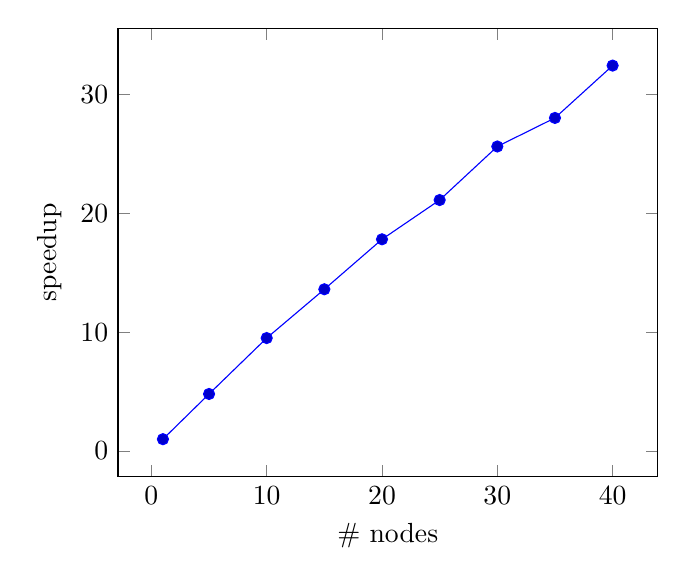
\begin{tikzpicture}
	\begin{axis}[xlabel=\# nodes,ylabel=speedup]
	\addplot coordinates {
		(1, 1)
		(5, 4.8)
		(10, 9.5)
		(15, 13.6)
		(20, 17.8)
		(25, 21.1)
		(30, 25.6)
		(35, 28.0)
		(40, 32.4)
	};
	\end{axis}
	\end{tikzpicture}
	\caption{Observed speedup when traversing the GIT fan with varying numbers of compute nodes.}
	\label{graph:traversal_speedup}
\end{figure}

\begin{figure}[t]
	\centering
	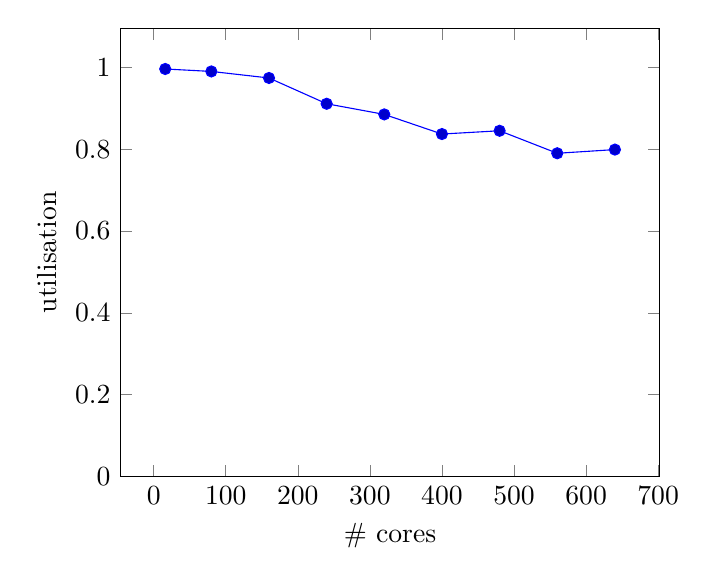
\begin{tikzpicture}
	\begin{axis}[xlabel=\# cores,ylabel=utilisation,ymin=0]
	\addplot coordinates {
		(16, 0.996)
		(80, 0.990)
		(160, 0.974)
		(240, 0.911)
		(320, 0.885)
		(400, 0.837)
		(480, 0.845)
		(560, 0.790)
		(640, 0.799)
	};
	\end{axis}
	\end{tikzpicture}
	\caption{Observed utilisation when traversing the GIT fan with varying numbers of compute nodes.}
	\label{graph:traversal_utilisation}
\end{figure}

\begin{figure}[t]
	\centering
	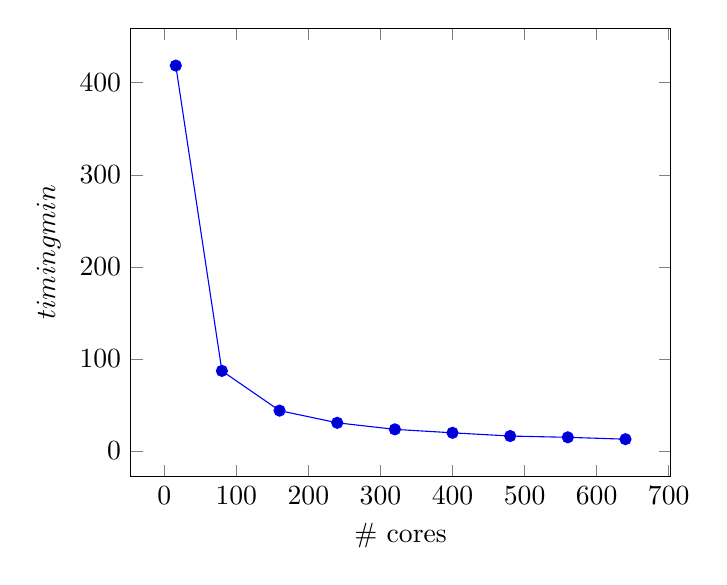
\begin{tikzpicture}
	\begin{axis}[xlabel=\# cores,ylabel=$\faktor{\text{timing}}{\text{min}}$]
	\addplot coordinates {
		(16, 418.5950)
		(80, 87.0672)
		(160, 43.9218)
		(240, 30.6985)
		(320, 23.5702)
		(400, 19.8228)
		(480, 16.3206)
		(560, 14.9239)
		(640, 12.9088)
	};
	\end{axis}
	\end{tikzpicture}
	\caption{Required computation time when traversing the GIT fan with varying numbers of compute nodes.}
	\label{graph:traversal_timing}
\end{figure}